\section{FORMAT OF THE MANUSCRIPT}
\label{sec:format}

\subsection{Reference Number}
Place the paper ID number, which will be announced on the received authors notification, at the top right corner of the header in a bold type, replace the ``\#\#\#'' in the header of this document with the paper ID number. The paper ID number should be followed by a page number (for example, ``\textbf{154, Page 1}'' for the first page). Please repeat this procedure for the second page, as they have different header layouts.

\subsection{Manuscript Title}
Center the manuscript title with font size of 14-point bolded with a blank line below the title.

\subsection{Authors}
All authors should be listed by their full name with the family name appearing last, i.e., how the name is written in English (e.g., Yu Li Cho, John Smith, Tae-yong Kim). The affiliation of the corresponding author should be given first. The affiliation and contact information of all co-authors should be listed as well. When necessary, asterisks should be used to indicate which affiliation goes with which author. The affiliation(s) should be centered and in upper/lower case letters. The different parts of the affiliation(s) should be separated by commas, and if more than one line is necessary, the different lines should be of about the same length.

\subsection{Number of Pages}
The entire manuscript (i.e., text, figures, tables, bibliography, etc.) \textbf{must be no more than 12 pages long} including graphs, tables and figures. Any manuscript having excess pages will not be accepted. 

\subsection{Text Format}
Times or Times New Roman font type \textbf{MUST} be used for any text in the document including captions, footnotes, and header information. All text has to be single spaced, black, and in 11-point type. All paragraphs must be single-spaced with a double space between each paragraph. The paragraph format is “justified”. If manuscript is prepared in the Asian format, please indicate in Page Set Up “No Grid Lines”. Asian single spacing appears as 1 1/2 spacing in Western formats.  Paragraphs are not to be indented. Use single-line spacing between lines except where symbols or equations require 1 1/2 line spaces.

\subsection{Paper Size and Margins}
Authors are asked to provide the manuscript in A4 (21cm x 29,7cm) following the margin settings explained in this section.

\textbf{IMPORTANT:} All text of the manuscript must be located within A4 paper format page. The margins are given in \cref{tab:margins}. All margins (top, bottom, left and right) have to be set at 2.54 cm.

\begin{table}[h!]
    \centering
    \caption{Page margins for manuscripts}
    \begin{tabular}{cllll}
        \toprule 
        Margin Position & Top & Bottom & Left & Right \\
        \midrule 
        A4 & \SI{2.54}{cm} & \SI{2.54}{cm} & \SI{2.54}{cm} & \SI{2.54}{cm} \\
        \bottomrule
    \end{tabular}
    \label{tab:margins}
\end{table}

\subsection{Format of Citations}
Within the text of the manuscript, bibliographical sources are to be cited by giving the last name(s) of the author(s) and the year of publication. The year should always be in parentheses. The two possibilities are illustrated as follows:
    
    \citet{Janna1986} showed that the blend was azeotropic.

or:	It was shown that the blend was azeotropic \citep{Janna1986}.

When there are two authors, the names of both should be cited, e.g.:

	\citet{Herbe1997} observed that the blend was azeotropic.
 
or:	It was observed that the blend was azeotropic \citep{Herbe1997}.

When there are three authors or more, only the lead author of the source should be cited. The names of the other authors should be designated by et al. in italics, e.g.:

	\citet{Hofmann2021} observed that the blend was azeotropic.
 
or:	It was observed that the blend was azeotropic \citep{Hofmann2021}.

When the same author and the same year of publication are cited from more than one source, the sources should be distinguished in the text by adding the small letter ``a'' to the year of publication of the first source cited, ``b'' for the second source, and so on, i.e.,
	
\citet{Tsatsaronis1985a} discovered ... and further on in the text:	\citet{Tsatsaronis1985b} also pointed out  that ...

\subsection{Figures and Tables}
Each table must be numbered, with the caption centered above the table and table number in \textbf{bold} as shown in \Cref{tab:margins}. Each figure must be numbered, with the caption centered below the figure and figure number in \textbf{bold} as shown in \Cref{fig:diagram}. Figures and tables should be incorporated into the main body of the text. It is best to position them at the top or bottom of a page and to leave one blank line to separate them from the rest of the text. Authors have to make sure that all tables and figures appear in their entirety on one page. All tables and figures must be sharp and clear. We recommend a resolution of least 300 dpi. All axis and data series must be labeled correctly. All text within the table and diagrams should be in \textbf{English}. 

\begin{figure}[h!]
    \centering
    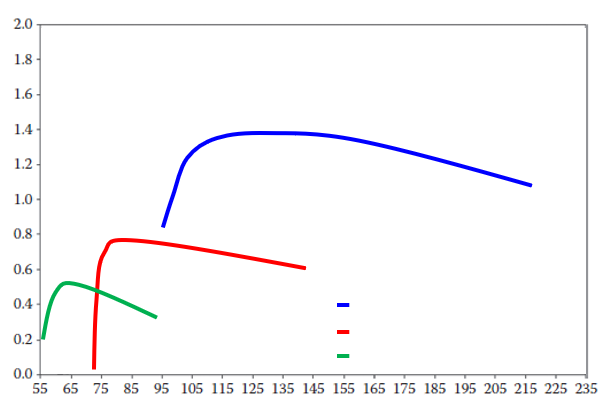
\includegraphics[scale=0.6]{figures/diagram.png}
    \caption{Lorem ipsum dolor sit amet}
    \label{fig:diagram}
\end{figure}

\subsection{Format of Equations}
Equations are to be centered, numbered in order (i.e., (1), (2), (3), etc.) on the right-hand side of the page and cited in the text with its number, e.g., ``... as listed in \Cref{eq:fn+an}”. Use 1.5 spacing, if necessary, for equations.  

Symbols used in equations should be explained directly below the equation in which they first appear or in a nomenclature section at the end of the manuscript. E.g., a method \citep{Cheap1986} to estimate the cost of attending meetings is given in \Cref{eq:fn+an}. Formatting of equations has to be checked before submittal of the manuscript.

\begin{equation}
    C=FN_p+AN_n
    \label{eq:fn+an}
\end{equation}

\subsection{Units Format}
SI units only.

\subsection{Footer and Page Numbering}
Authors are asked to include the one-line footer centered on each page of their manuscript. The footer has to be placed \SI{1.27}{cm} from the bottom edge of the page. The required footer is included in the footer of the author template of this conference. The page number should be appended to the paper ID number in the header.
